\documentclass[tikz,border=10pt]{standalone}
\usepackage{tikz}
\usetikzlibrary{positioning}
\usepackage{tikz-feynman}
\begin{document}

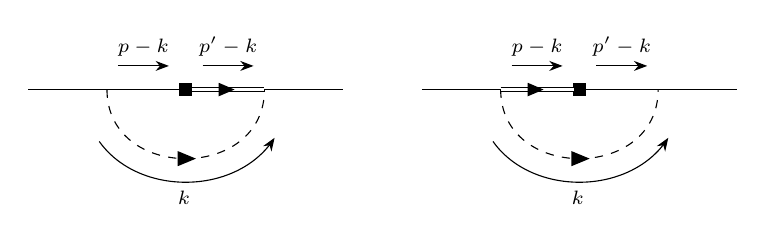
\begin{tikzpicture}[
		decuplet/.style={ % 自定义一个重子的双线
				double distance=1pt,
				postaction={decorate}, decoration={
						markings, mark=at position .6 with {
								\arrow{Triangle[angle=40:1pt 3]}
							},
					}
			}
	]
	\begin{feynman}
		% fig trans mag left
		\vertex (i1) at (0,0);
		\vertex[right =1cm  of i1] (i2);
		\vertex[right =2cm  of i1,square dot,anchor=center] (i3){};
		\vertex[right =3cm  of i1] (i4);
		\vertex[right =4cm  of i1] (i5);
		\node[above =0.5 of i5] {};
		%  fig trans mag right
		\vertex[right =5cm  of i1] (j1);
		\vertex[right =1cm  of j1] (j2);
		\vertex[right =2cm  of j1,square dot,anchor=center] (j3){};
		\vertex[right =3cm  of j1] (j4);
		\vertex[right =4cm  of j1] (j5);
		\node[above =0.5 of j5] {};
		% 对各个顶点连线
		\diagram*{
		{[edge=plain]
		(i2) --[momentum={\scriptsize \(p-k\)} ]  (i3) --
		[momentum={\scriptsize \(p^{\prime}-k\)}] (i4),
		(j2) --[momentum={\scriptsize \(p-k\)} ]  (j3) --
		[momentum={\scriptsize \(p^{\prime}-k\)}] (j4),
		},
		{[edge=plain]
				(i1) -- (i2)--(i3),(i4)-- (i5),
				(j1) -- (j2),(j3)--(j4)-- (j5),
			},
		% 介子连线
		{[edge= charged scalar]
		(i2) --[half right, momentum'={\scriptsize \(k\)}](i4),
		(j2) --[half right, momentum'={\scriptsize \(k\)}](j4),
		}
		};
		%% 添加重子双线
		\draw[decuplet]	 (i3) -- (i4);
		\draw[decuplet]	 (j2) -- (j3);
	\end{feynman}
\end{tikzpicture}

\end{document}

